\section{Continuity}
In this section, we talk about $ f:E \to \mathbb{C}  $ where $ E \subseteq \mathbb{C}  $.
\subsection{Continuity of real- and complex-valued functions}
\subsubsection{Definitions}

There are two definitions for continuity.

\begin{definition}[Sequence definition]
    $f$ is continuous at $ a\in E $ if for every sequence $ z_n\in E\to a $, we have $ f(z_n)\to f(a) $.
\end{definition}

\begin{definition}[Epsilon-delta definition]
    $f$ is continuous at $a\in E$ if given $ \epsilon>0 $, $ \exists \delta>0 $ such that if $ z\in E, |z-a|<\delta $, then $ |f(z)-f(a)|<\epsilon $.
\end{definition}

\begin{sprop}
    Sequence definition $ \Longleftrightarrow $ Epsilon-delta definition.
\end{sprop}
\begin{proof}
    ($ \Leftarrow $) We know that $ \forall \epsilon,\exists \delta: |z-a|<\delta \Rightarrow |f(z)-f(a)|<\epsilon $. Let $ z_n\in E \to a $, then $ \exists n_0 $ such that $ \forall n\ge n_0 $, we have
    \[
        |z_n-a|<\delta \Longrightarrow |f(z_n)-f(a)|<\epsilon \Longrightarrow f(z_n) \to f(a).
    \]

    ($ \Rightarrow $) Assume that $ f(z_n)\to f(a) $ whenever $E\ni z_n\to a $. Suppose $f$ is \textit{not} continunous at $a$ by definition 2.2. Then
    \[
        \exists \epsilon>0, \forall \delta>0, \exists z\in E: |z-a|<\delta,\text{ but } |f(z)-f(a)|\ge \epsilon.
    \]
    Take $ \delta=1/n $, then $ \exists  z_n $ such that $ |z_n-a|<1/n $ and $ |f(z_n)-f(a)|\ge \epsilon $. Clearly $ z_n\to a $, but $ f(z_n)\nrightarrow f(a) $, \#.
\end{proof}

\subsubsection{Arithmetic of continuous functions}

\begin{proposition}\label{prop:2.1}
    Let $a\in E$ and $ g,f:E\to \mathbb{C} $ be continuous at $a$. Then so are the functions $ f+g $, $fz$ and $\lambda f$ for any constant $ \lambda\in \mathbb{C} $. In addition, if $f(z)\neq 0 \forall z\in \mathbb{C} $, then $ 1/f $ is continuous at $a$.
\end{proposition}
\begin{proof}
    It becomes obvious if we use the sequence definition and by lemma \ref{lma:1.1}.
\end{proof}

\begin{example}
    $ f(z)=z $ is continuous. Thus every polynomial is continuous at every point, and every rational function is continuous at every point on \textit{domain}.
\end{example}

\begin{note}
    We say that $f$ is continuous on $E$ if $ \forall a\in E $, $f$ is continuous at $a$.
\end{note}
\begin{remark}
    Still it is instructive to prove proposition \ref{prop:2.1} from $ \epsilon $-$ \delta $ language.
\end{remark}

\begin{theorem}\label{thm:2.2}
    Let $f:A\to \bbC$ and $g:B\to \bbC$ be 2 functions such that $ f(A) \subseteq B $. Suppose $f$ is continuous at $a\in A$ and $g$ is continuous at $f(a)\in B$, then $ g \circ f:A\to \mathbb{C}  $ is continuous at $a$.
\end{theorem}
\begin{proof}
    Take $ z_n\to a\in A $. By assumption, $ B\ni w_n:=f(z_n)\to f(a) $ so $ g(w_n)=g(f(z_n))\to g(f(a)) $, as expected.
\end{proof}

\begin{example}
    Let $ f:\mathbb{R} \to \mathbb{R}  $ be such that
    \[
        f(x) = \begin{cases}
            \sin \left( 1/x \right) & \text{if } x\neq 0, \\
            0                       & \text{if }x=0.      \\
        \end{cases}
    \]
    Note that $ \sin x $ is continuous(to be proved later). If $x\neq 0$ then $f$ is continuous at $x$. Take $ x_n = 1/((2n+1/2)\pi) $, then $ f(x_n)\equiv 1\nrightarrow 0 $, so $f$ is discontinuous at 0.

    Now let $g:\mathbb{R} \to \mathbb{R} $ be such that
    \[
        g(x)=\begin{cases}
            x\sin \left( 1/x \right) & \text{if } x\neq 0, \\
            0                        & \text{if }x=0.      \\
        \end{cases}
    \]
    $g$ is continuous at 0 since taking $ x_n\to 0 $, we have $ |f(x_n)|\le |x_n| $ since $ |\sin x|\le 1 $(to be proved later). Hence $ f(x_n)\to 0 $.
\end{example}

\begin{example}[Dirichlet function]
    Consider 
    \[
        D(x) = \begin{cases}
        1 &\text{if }x\in \mathbb{Q}, \\
        0 &\text{if }x\in \bbQ^\complement.\\
        \end{cases} 
    \]
    It is discontinuous at every point. Indeed, if $x\in \bbQ$, take $x_n\to x$ with $ x_n\in \bbQ^\complement,\forall n $, then $ D(x_n)\equiv 0 \nrightarrow D(x)=1 $. Similar for $ x\in \bbQ^\complement $.
\end{example}

\subsection{Limit of a function}
\begin{definition}[Limit point]
    Let $ E\in \mathbb{C} $ and $ a\in \mathbb{C} $. We say $a$ is a \textbf{limit point} of $E$ if $ \forall \delta>0, \exists z\in E: 0<\left| z-a \right| <\delta $.
    \begin{center}
        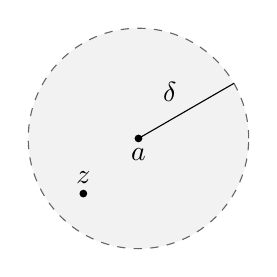
\begin{tikzpicture}[scale=0.7]
            \filldraw[color=black!60, fill=black!5, dashed](0,0) circle (2);
            \fill [black] (0,0) circle (2pt) node [below] {$a$};
            \draw (0,0) -- (1.732,1) node [pos=0.5,above left] {$ \delta $};
            \fill [black] (-1,-1) circle (2pt) node [above] {$z$};
        \end{tikzpicture}
    \end{center}
\end{definition}
\begin{remark}
    $a$ is a limit point if and only if $ \exists z_n\in E $ such that $ z_n\to a $ and $ z_n\neq a $ for all $n$. Can check this is equivalent to the definition.
\end{remark}

\begin{definition}[Limit of a function]
    $ f:E\to \mathbb{C} $ and let $ a\in \mathbb{C} $ be a limit point of $E$.We say 
    \[
        \lim_{z \to a} f(z) = L \Longleftrightarrow \forall \epsilon>0, \exists \delta>0, \forall \left| z-a \right| <\delta: \left| f(z)-L \right| \epsilon.
    \]
    Equivalently,
    \[
        \lim_{z \to a} f(z)=L \Leftrightarrow \forall (z_n)_{n\in\bbN} \subseteq E, z_n\neq a \land z_n\to a: f(z_n)\to L.
    \]
\end{definition}

\begin{remark}
    Immediate from definition, If $ a\in E $ is a limit point, then $ \lim_{z \to a} f(z)=f(a) $ if and only if $f$ is continuous at $a$. If $a$ is isolated(i.e. $a\in E$ and is not a limit point), continuity of $f$ at $a$ is trivially true.
\end{remark}

\begin{sprop}
    Limits of functions have similar properties to limits of sequences.
    \begin{enumerate}
        \item It is unique.
        \item $f(z)g(z)\to AB$.
        \item If $B\neq 0$, $ f(z)/g(z)\to A/B $.
    \end{enumerate}
\end{sprop}
Proof is exercise.

\subsection{Intermediate value theorem}
\begin{theorem}[Intermediate value theorem]\label{thm:intermediate value theorem}
    If $ f:[a,b]\to \mathbb{R}  $ is continuous and $ f(a)\neq f(b) $, then $f$ takes every value bewteen $f(a)$ and $f(b)$.
\end{theorem}
\begin{proof}
    Wlog suppose $ f(a)<f(b) $. Take $ \eta\in (f(a),f(b)) $. Let 
    \[
        S = \{x\in [a,b]:f(x)<\eta \}.
    \]
    Note that $a\in S$ and $S$ is clearly bounded above (by $b$), so $ \exists c = \sup S\le b $. 
    
    Claim that $f(c)=\eta$. Indeed, by definition of supremum, $ \forall n $, $ \exists x_n\in S$ such that $ c-\frac{1}{n}<x_n\le c $. Clearly $x_n\to c$. Since $ x_n\in S, f(x_n)<\eta $. By continuity of $f$, $f(x_n)\to f(c)\le \eta$. 

    Now observe that $ c\neq b $, otherwise we have $ f(b)\le \eta $ which is impossible. Then for $n$ large, $ c+\frac{1}{n}\in [a,b] $ and $ c+\frac{1}{n}\to c $. By continuity, $ f(c+\frac{1}{n})\to f(c)\ge \eta $.

    Therefore $ f(c)=\eta $, as claimed.
\end{proof}
\begin{remark}
    The theorem is very useful for finding zeros of fixed points.
\end{remark}

\begin{example}[Existence of the $N$th root of a positive real number]
    Let $ f(x)=x^N, x\ge 0 $. $f$ is continuous and pick $y>0$. By intermediate value theorem, $f$ takes every value $ [0,f(y)+1] $. Therefore $ \exists x, x^N=y $. If $ d^N=y,d\neq x $, wlog suppose $d<x$ so $ d^N<x^N \Rightarrow y<y $ which is absurd. Hence it is unique. 
\end{example}